\usepackage{amsfonts,epsfig,float,multicol,txfonts,framed,calc,array,xcolor,wrapfig}
\usepackage[Lenny]{fncychap}
\usepackage{fancyhdr}
\fancyhead[RO,LE]{\thepage}
\fancyhead[LO]{\rightmark}
\fancyfoot{}
\definecolor{shadecolor}{RGB}{204,204,255}
\definecolor{ggbBrown}{HTML}{993300}
\definecolor{ggbGreen}{HTML}{006400}

%%%%%%%%%%%%%%%%%%%%%%%%%%%%%%%%%%%
% Create counters for use in book %
%%%%%%%%%%%%%%%%%%%%%%%%%%%%%%%%%%%
\newcounter{pagegrab}
\newcounter{enumigrab}
\newcounter{sagemathcell}
\setcounter{sagemathcell}{1}

%%%%%%%%%%%%%%%%%%%%%%%%%%%%
% Part page without number %
%%%%%%%%%%%%%%%%%%%%%%%%%%%%
\newcommand{\mypart}[1]{
  \setcounter{pagegrab}{\thepage}
  \pagenumbering{gobble}
  \part{#1}
  \pagenumbering{arabic}
  \stepcounter{pagegrab}
  \stepcounter{pagegrab}
  \setcounter{page}{\thepagegrab}
}

\newcommand{\sagecell}[1]{\href{#1}{
\includegraphics[height=12pt]{SageMathCell} \thesagemathcell}\stepcounter{sagemathcell}}

%%%%%%%%%%%%%%%%%%%%%%%%%%%%%%%%%%%%%%%%%%%%%%%%%%%%%%%%%
% Redefine \boxed                                       %
% will put a green box around a mathematical expression %
%%%%%%%%%%%%%%%%%%%%%%%%%%%%%%%%%%%%%%%%%%%%%%%%%%%%%%%%%
\renewcommand{\boxed}[1]{\text{\fboxsep=.2em{\color{green}\fbox{\color{black}\m@th$\displaystyle#1$}}}}

%%%%%%%%%%%%%%%%%%%%%
% Define Bold \cdot %
%%%%%%%%%%%%%%%%%%%%%
\newcommand{\bcdot}{\boldsymbol\cdot}

%%%%%%%%%%%%%%%%%%%%%%%%%%%%%%%%%%%%%%%
% Define dictionary style accent mark %
%%%%%%%%%%%%%%%%%%%%%%%%%%%%%%%%%%%%%%%
\newcommand{\dictacc}{\raisebox{2pt}{$ \,\prime\, $}}

%%%%%%%%%%%%%%%%%%%%%%%%%%%%%%%%%%%%%%
% Sage and GeoGebra Logo definitions %
%%%%%%%%%%%%%%%%%%%%%%%%%%%%%%%%%%%%%%
\graphicspath{{$HOME/Documents/scsu/Book-Linear/figures/}}
\newcommand{\sage}{\href{https://sagecell.sagemath.org/}{\includegraphics[height=12pt]{sageLogo}}}
\newcommand{\geogebra}{\href{https://www.geogebra.org/calculator}{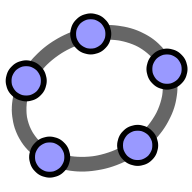
\includegraphics[height=12pt]{geogebraLogo}}}

%%%%%%%%%%%%%%%%%%%%%%%%
% Exercises definition %
%%%%%%%%%%%%%%%%%%%%%%%%
\newcommand{\startexercises}{\begin{multicols}{2}\begin{small}}
\newcommand{\finishexercises}{\end{small}\end{multicols}}

%%%%%%%%%%%%%%%%%%%%%%%%%
% Digression definition %
%%%%%%%%%%%%%%%%%%%%%%%%%
\newlength\myRightmargin
\newlength\myLeftmargin
\newcounter{thecrumpet}
\newenvironment{digression}[1]
  {%\bigskip%
  \begin{shaded*}
   \begin{list}{}%
   {\global\addtolength\myLeftmargin{\parindent}%
   \global\addtolength\myRightmargin{\parindent}%
   \setlength{\leftmargin}{\myLeftmargin}%
   \setlength{\rightmargin}{\myRightmargin}%
   \setlength{\listparindent}{\parindent}}%
   \item\relax%
   \hrule%
   \refstepcounter{thecrumpet}
   \begin{center}\textbf{Crumpet \arabic{thecrumpet}:} #1\end{center}%
   \smallskip\hrule\medskip%
   \begin{small}\noindent{}}
  {\end{small}%
   \medskip%
   \hrule%
   \end{list}
   %\bigskip%
   \end{shaded*}
   \global\addtolength\myLeftmargin{-\parindent}%
   \global\addtolength\myRightmargin{-\parindent}}

%%%%%%%%%%%%%%%%%%%%%%%%%%%%%%%%%%%%%%%%%%%%%%%%%%%%
% Markers for exercises with solutions and answers %
%%%%%%%%%%%%%%%%%%%%%%%%%%%%%%%%%%%%%%%%%%%%%%%%%%%%
%\newcommand{\hasasolution}{{\color{blue}${}^{[\mathbb{S}]}$}}
\newcommand{\hasasolution}{\enspace{\color{blue}${[\mathbb{S}]}$}-}
\newcommand{\haspartwithsolution}{{\color{gray}${}^{[\mathbb{S}]}$}}
%\newcommand{\hasananswer}{{\color{blue}${}^{[\mathbb{A}]}$}}
\newcommand{\hasananswer}{\enspace{\color{blue}${[\mathbb{A}]}$}-}
\newcommand{\haspartwithanswer}{{\color{gray}${}^{[\mathbb{A}]}$}}

%%%%%%%%%%%%%%%%%%%%%%%%%%%%%%%%%%%%%%%%%%%
% Raise graphic for insertion into a list %
%%%%%%%%%%%%%%%%%%%%%%%%%%%%%%%%%%%%%%%%%%%
\newlength{\picheight}
\newcommand{\raisepic}[1]{
  \setlength{\picheight}{\heightof{#1}}
  \addtolength{\picheight}{-\baselineskip}
  \raisebox{-\picheight}{#1}
}
  
  
% Possible title page styles
% complements of titlepages.pdf
% code copied from titlepages.tex

\ifpdf
  \usepackage{pdfcolmk}
\fi

\providecommand*{\FSfont}[1]{}%    kills special font selections
\providecommand*{\wb}[2]{}%    probably kills Web-O-Mints (and some layouts?)
\providecommand{\HUGE}{\Huge}% if not using memoir

\newcommand*{\plogo}{\fbox{$\mathcal{PL}$}}

\newlength{\tpheight}\setlength{\tpheight}{0.9\textheight}
\newlength{\txtheight}\setlength{\txtheight}{0.9\tpheight}
\newlength{\tpwidth}\setlength{\tpwidth}{0.9\textwidth}
\newlength{\txtwidth}\setlength{\txtwidth}{0.9\tpwidth}
\newlength{\drop}

\newcommand*{\titleHGP}{\begingroup% Handy Guide to Papermaking
\drop=0.1\txtheight
\begin{minipage}[t]{0.05\txtwidth}
  \color{Red}
  \rule{6pt}{\txtheight}
\end{minipage}
\hspace{0.05\txtwidth}
\begin{minipage}[t]{0.6\txtwidth}
  \vspace*{\drop}
  {\Large LEON Q. BRIN} \\
  \rule{0.9\txtwidth}{1pt} \par
  \vspace{3\baselineskip}
  {\noindent\Huge\bfseries Tea Time\\[.15\baselineskip]Linear\\[.15\baselineskip]Algebra} \par
  \vspace{2\baselineskip}
  {\Large\itshape Experiences in Mathematics} \par
  \vspace{6.5\baselineskip}
  {\scshape the secnd in a series of tea time textbooks} \par
  \vspace{\baselineskip}
  \rule{0.9\txtwidth}{1pt} \par
  \vspace{\baselineskip}
  {\Large SOUTHERN\\[.15\baselineskip]CONNECTICUT\\[.15\baselineskip]STATE\\[.15\baselineskip]UNIVERSITY}
\end{minipage}
%\hfill
\hspace{0.23\txtwidth}
\begin{minipage}[t]{0.15\txtwidth}
  {\color{Red} 
  \FSfont{5fh}% FontSite Fette Gotisch
  \HUGE
  \vspace{3.3\baselineskip}
  $\mathfrak{C}$ \\[.32\baselineskip]
  $\mathfrak{C}$ \\[.32\baselineskip]
  $\mathfrak{-}$ \\[.32\baselineskip]
  $\mathfrak{B}$ \\[.32\baselineskip]
  $\mathfrak{Y}$ \\[.32\baselineskip]
  $\mathfrak{-}$ \\[.32\baselineskip]  
  $\mathfrak{S}$ \\[.32\baselineskip]
  $\mathfrak{A}$
}\par
%  \vspace{4\baselineskip}
%  {\Large 2014}
\end{minipage}
\endgroup}

\newcommand*{\titleGM}{\begingroup% Gentle Madness
\drop = 0.1\txtheight
%\vspace*{\baselineskip}
\vfill
  \hbox{%
  \hspace*{0.2\txtwidth}%
  \rule{1pt}{\txtheight}
  \hspace*{0.05\txtwidth}%
%\fbox{%
\parbox[b]{0.75\txtwidth}{
  \vbox{%
    \vspace{\drop}
    {\noindent\HUGE\bfseries Tea Time\\[0.5\baselineskip]Linear Algebra}\\[2\baselineskip]
    {\Large\itshape Experiences in Mathematics}\\[4\baselineskip]
    {\Large LEON Q. BRIN}\par
    \vspace{0.5\txtheight}
    {\noindent Southern Connecticut State University}\\[\baselineskip]
    }% end of vbox
}% end of parbox
%}% end of fbox
  }% end of hbox
\vfill
\null
\endgroup}

\newcommand*{\titleTMB}{\begingroup% Three Men in a Boat
\drop=0.1\txtheight
\centering
\settowidth{\unitlength}{\LARGE TEA TIME LINEAR ALGEBRA}
\vspace*{\baselineskip}
{\large\scshape LEON Q. BRIN}\\[\baselineskip]
\rule{\unitlength}{1.6pt}\vspace*{-\baselineskip}\vspace*{2pt}
\rule{\unitlength}{0.4pt}\\[\baselineskip]
{\LARGE TEA TIME LINEAR ALGEBRA}\\[\baselineskip]
{\itshape experiences in mathematics}\\[0.2\baselineskip]
\rule{\unitlength}{0.4pt}\vspace*{-\baselineskip}\vspace{3.2pt}
\rule{\unitlength}{1.6pt}\\[\baselineskip]
{\large\scshape the second in a series of tea time textbooks}\par
\vfill
{\large\scshape southern connecticut state university}\\[\baselineskip]
{\small\scshape 2021}\par
\vspace*{\drop}
\endgroup}

\newcommand*{\titleGP}{\begingroup% Geometric Modeling
\drop=0.1\txtheight
\centering
\vspace*{\baselineskip}
\rule{\txtwidth}{1.6pt}\vspace*{-\baselineskip}\vspace*{2pt}
\rule{\txtwidth}{0.4pt}\\[\baselineskip]
{\LARGE TEA TIME\\[0.3\baselineskip]LINEAR ALGEBRA}\\[0.2\baselineskip]
\rule{\txtwidth}{0.4pt}\vspace*{-\baselineskip}\vspace{3.2pt}
\rule{\txtwidth}{1.6pt}\\[\baselineskip]
\scshape
Experiences in Mathematics \\
Location, date from--to\par
\vspace*{2\baselineskip}
Edited by \\[\baselineskip]
{\Large FIRST EDITOR \\ SECOND EDITOR \\ THIRD EDITOR\par}
{\itshape Organisation \\ Address\par}
\vfill
\plogo\\
{\scshape year} \\
{\large THE PUBLISHER}\par
\endgroup}

\newcommand*{\titlePP}{\begingroup% Printing Poetry
\newlength{\rtab}
\setlength{\rtab}{.25in}
\newlength{\titlewidth}
\settowidth{\titlewidth}{\textbf{\HUGE TEA TIME LINEAR ALGEBRA}}
\definecolor{MidnightBlue}{HTML}{282a65}
\FSfont{5jr}% FontSite Jenson Recut (Centaur)
\drop=0.1\txtheight
\vspace*{\drop}
\begin{raggedleft}
\ \\
{\color{MidnightBlue}\rule{1.02\titlewidth}{3pt}}\hspace{\rtab}\phantom{|} \\[1.25\baselineskip]
\textbf{\HUGE\color{MidnightBlue} TEA TIME LINEAR ALGEBRA}\hspace{\rtab}\phantom{|} \\[.5\baselineskip]
\textit{\LARGE\color{MidnightBlue} Explorations in Mathematics}\hspace{\rtab}\phantom{|} \\[1.5\baselineskip]
{\LARGE Leon Q. Brin}\hspace{\rtab}\phantom{|} \\[\baselineskip]
{\color{MidnightBlue}\rule{1.02\titlewidth}{3pt}}\hspace{\rtab}\phantom{|} \\[.5\baselineskip]
{the second in a series of tea time textbooks}\hspace{\rtab}\phantom{|} \par
\end{raggedleft}
\vfill
\begin{center}
{\Large Southern Connecticut State University}
\end{center}
\vspace*{\drop}
%\mbox{}
\endgroup}
